\chapter{Uncertainty Quantification in Dynamical Systems}
\label{chap:uq}

Consider a $n$-dimensional coupled dynamical system defined by the following Stochastic Differential Equation (SDE)
\begin{equation}
\label{stochdyn}
\dot{\mathbf{x}}_t = f(\mathbf{x}_t)  \hspace{5 mm} \textbf{x}_{t_0} = \textbf{x}_0
\end{equation}

\noindent where $\textbf{x} \in \mathbb{R}^n$ is the state variable, $f(x)$ is an $n$-dimensional vector of deterministic square integrable functions $f = [f_1,f_2,\ldots,f_n]$, with  $f: \mathbb{R}^n \times \mathbb{R}  \rightarrow \mathbb{R}^n$. Here $\mathbf{x}_t = \lbrace\mathbf{x}(t,\omega) , t \in [0,\infty) , \omega \in \Omega_{\mathbf{x}} \rbrace$ is a stochastic process defined on the probability space $(\Omega_\mathbf{x},\mathcal{F}_\mathbf{x},P_\mathbf{x})$ and
\begin{equation}
\textbf{x}_t :([0,\infty)\times \Omega_\mathbf{x}, \mathcal{B}([0,\infty)), \mathcal{F}_\mathbf{x}) \rightarrow (\mathbb{R}^n, \mathcal{B}(\mathbb{R}^n))
\end{equation}

Solution to Equation~\ref{stochdyn} admits is given by the nonlinear transformation $\textbf{x}_t = \phi^t(\mathbf{x}_0)$, where the deterministic flow is given by:
\begin{equation}
\label{stochflow}
\phi : \mathbb{R} \times \Omega_\mathbf{x}  \rightarrow \mathbb{R}^n
\end{equation}

Here the operation $\phi^t(x)$ is bijective, and satisfies (i) $\phi^0(\textbf{x}_0) = \textbf{x}_0$ and (ii) $\phi^{t+s}(\textbf{x}_0) = \phi^t(\phi^s(\textbf{x}))$, where $t \in \mathbb{R}$ is referred as time. Thus, the flow map $\phi^t(\mathbf{x}_0)$ is a random function depending on the initial distribution $\mathbf{x}_0$. 

\noindent In a given interval of time $t \in [0,T)$, a trajectory for a given initial condition $\textbf{x}_{0}$ at time $t = 0$ is defined as,

\begin{equation}
\label{gamma}
\gamma_{T,\textbf{x}_0} = \lbrace \phi^t(\textbf{x}_{0}) | t \in [0,T) \rbrace 
\end{equation}

\noindent An equilibrium point of the deterministic dynamical system with given flow velocity $f$, is defined as the point in the zero set of $f$ defined as,
\begin{equation}
\mathcal{Z} = \lbrace \tilde{x} \in \mathbb{R}^n | f(z) = 0 \rbrace
\end{equation}

The probability measure $P_{\textbf{x}_t}$ is characterized by the density function $p(\textbf{x}_t,t): \mathbb{R}^n \times \mathbb{R} \rightarrow [0,1]$ is a function of both $\textbf{x}_t$ and $t$, where,                     

\begin{equation}
\label{pdf_func}
P_{\textbf{x}_t} = P(\textbf{x}_t \leq \textbf{z}_t) = \int \int \ldots \int_{-\infty} ^{\textbf{z}_t} p(\tau,t) d\tau
\end{equation}

Our objective is to efficiently compute the statistical properties (say, first few moments) of state variable $\mathbf{x}_t = \phi^t(\mathbf{x}_0)$, given as:
\begin{equation}
\label{moments}
\begin{array}{l}
\mu_{t_k} = E[\mathbf{x}_{t_k}]  \\
\Sigma_{t_k} = E\left[(\mathbf{x}_{t_k} - \mu_{t_k})(\mathbf{x}_{t_k} - \mu_{t_k})'\right]
\end{array}
\end{equation}

\section{Moment Computation and Volume Integral}

\label{volume_integral}
As mentioned earlier, solution to system of high-dimensional ODEs requires solving simultaneous high-dimensional integrals. Let us consider an ODE $\dot{\textbf{x}}_t = f(\textbf{x}_t)$, $\textbf{x} \in \mathbb{R}^n$, represented by vector of deterministic functions $f = [f_1,f_2,\ldots,f_n]$, where $f_i:\mathbb{R}^n \rightarrow \mathbb{R}$, $i = 1$ to $n$. Similar to Equation~(\ref{stochflow}), the solution to this equation is given by the vector of functions $\phi^t(\textbf{x}_0) = [\phi^t(\textbf{x}_0)_1, \phi^t(\textbf{x}_0)_2, \ldots, \phi^t(\textbf{x}_0)_n]$, where $\textbf{x}_0$ is the initial condition. The solution $\textbf{x}_t = \phi^t(\textbf{x}_0)$ is defined for all $t \in \mathbb{R}$. The function $\phi^t(\textbf{x}_0)$ is obtained by solving the system of integral given as,

\begin{equation}
\label{integral_whole}
\mathbf{x_{t}} =  \phi^t(\mathbf{x}_0) = \mathbf{x}_0 + \int_0^t f(x_{\tau 1},x_{\tau 2},\ldots,x_{\tau n}) d \tau
\end{equation}

\noindent and the moment of an arbitrary function $\mathcal{G}$ similar to Equation~\ref{moments} can be written using the following volume integral,

\begin{equation}
\label{moment_whole}
E[\mathcal{G}(\textbf{x}_t)] = \int \int \ldots \int_{\Omega_{\textbf{x}}} \mathcal{G}(x_{t1},x_{t2},\ldots,x_{tn}) dP_{\textbf{x}}
\end{equation}


\section{Methods of Uncertainty Quantification}

UQ in high-dimensional dynamical systems involves propagation and computation of complex stochastic integrals involving the state variables. An analytical expression for the integrals in Equation~\ref{moment_whole} exists for only a few pdfs for a limited number of transformations. For arbitrary nonlinear transformations (such as Equation~\ref{integral_whole}), usage of numerical UQ techniques become the only possible solution. Any UQ method utilizes the definition of the pdf to generate sample points to compute the integral equation (Equation~\ref{integral_whole}). UQ methods studied in this dissertation is classified into two types: (i) Sampling-based methods and (ii) Collocation based methods. Given below is a review of some of the existing UQ methods. Review of Polynomial Chaos Expansion~\cite{xiu2002wiener} and related Galerkin projection methods~\cite{fletcher1984computational} are beyond the scope of this dissertation. 


\section{Monte Carlo Integration}

Integral computation as in Equation~\ref{moment_whole} can be based on random sampling or Monte Carlo (MC) sampling $\mathcal{X}_i$ of the pdf $p_\textbf{x} = dP_\textbf{x}$ and computation of the function value $\mathcal{G}(\mathcal{X}_i)$ for each random sample~\cite{fishman1996monte}. If there are $\mathcal{N}$ number of random samples, then Equation~\ref{moment_whole} can be computed as,

\begin{equation}
\label{monte_int}
E[\mathcal{G}(\textbf{x}_t)] = \int \int \ldots \int_{\Omega_{\textbf{x}}} \mathcal{G}(x_{t1},x_{t2},\ldots,x_{tn}) dP_{\textbf{x}} = \frac{
1}{\mathcal{N}} \sum_i^{\mathcal{N}} \mathcal{G}(\mathcal{X}_i)
\end{equation}

The integral in Equation~\ref{monte_int} is also referred to as Monte Carlo integral equation. The pdf $p_{\textbf{x}_t}(\bm{\tau})$ at any time $t$ is estimated from the evolution of the samples $\mathcal{X}_i$ via the propagation equations~\ref{stochdyn} and~\ref{stochflow}. Figure~\ref{montecarlo} shows a schematic of Monte Carlo based UQ method applied on an ODE. 

\begin{figure}[H]
\begin{center}
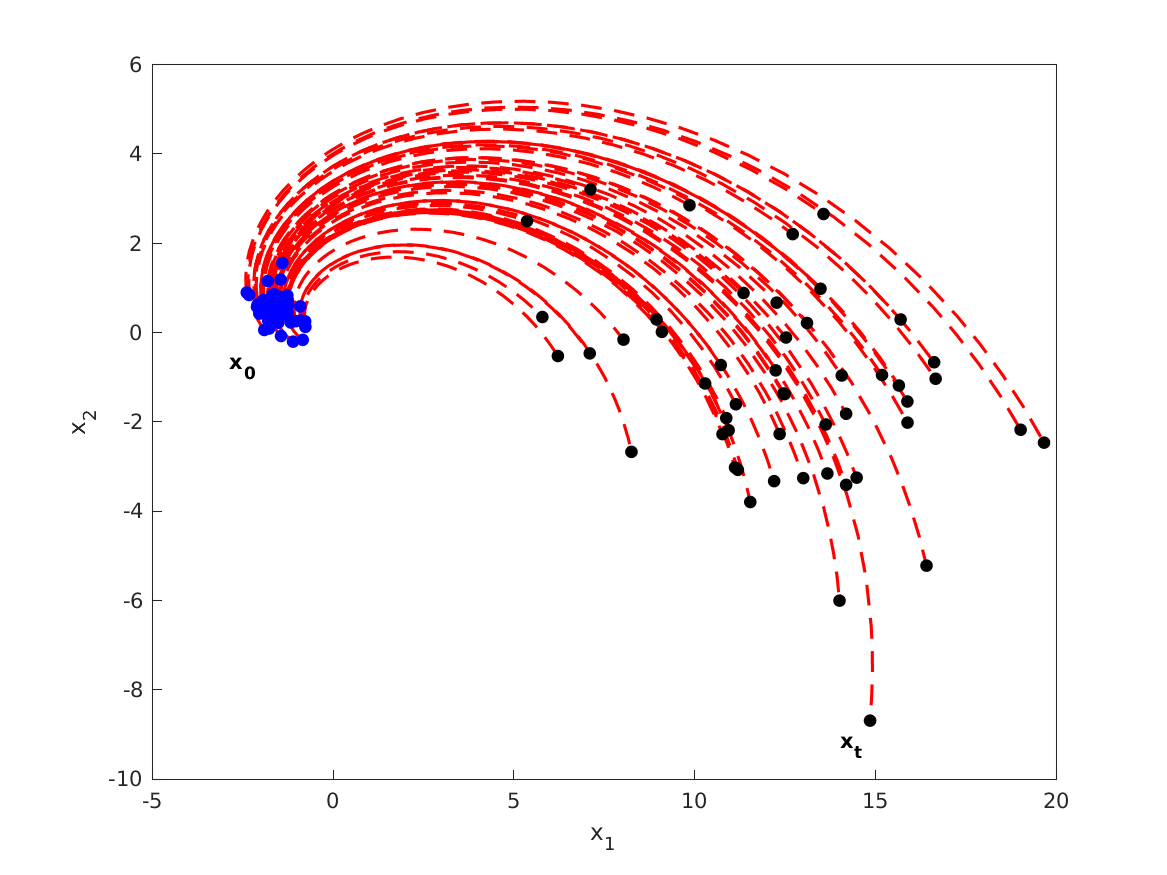
\includegraphics[scale=0.5]{figures/montecarlo}
\caption{Schematic of Monte Carlo simulation based UQ method applied on an ODE}
\label{montecarlo}
\end{center}
\end{figure}


The number of samples $\mathcal{N}$ and associated accuracies depends on the type of sampling methods employed. Standard sampling techniques refer to the generation of pseudo-random numbers. However, the convergence rate of the integral Equation~\ref{monte_int} can be estimated using the Central Limit Theorem as~\cite{stroud1971approximate} 

\begin{equation}
\epsilon_{\mathcal{N}} = \left(\frac{E[f^2]- E[f]^2}{\mathcal{N}}\right)^{1/2} 
\end{equation}

Figure~\ref{fig:monte_accuracy} shows the accuracy of MC sampling from an $n$-dimensional Gaussian random variable. The increase in estimation error shows a linear pattern with $n$. To reduce the error in convergence, different variance reduction techniques have been developed. These techniques use an underlying MC method and employ other deterministic techniques such as stratification, low discrepancy sequence generation to reduce the error in convergence. 


\begin{figure}[H]
\centering
\begin{subfigure}{0.45\textwidth}
\centering
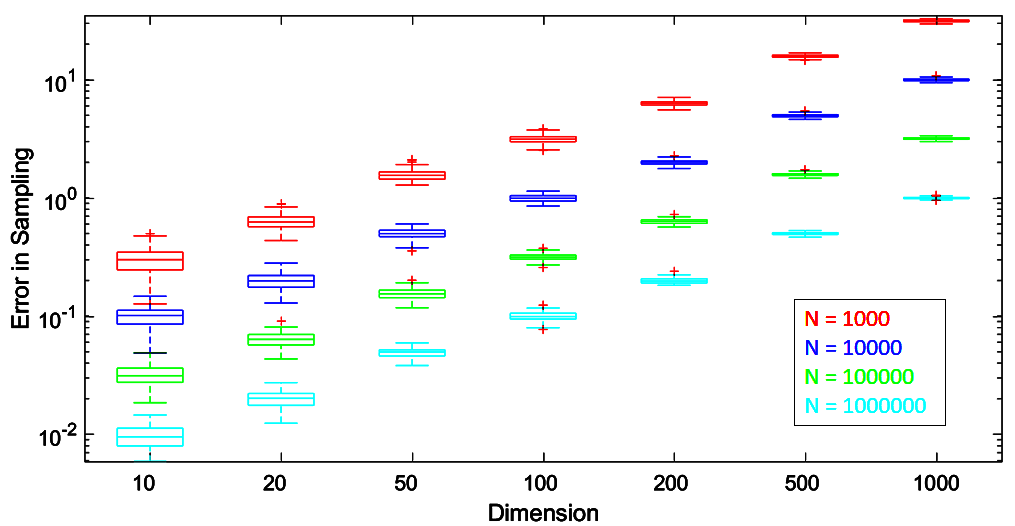
\includegraphics[width=\textwidth]{uq_figs/monte_log}
\caption{}
\end{subfigure}
\begin{subfigure}{0.45\textwidth}
\centering
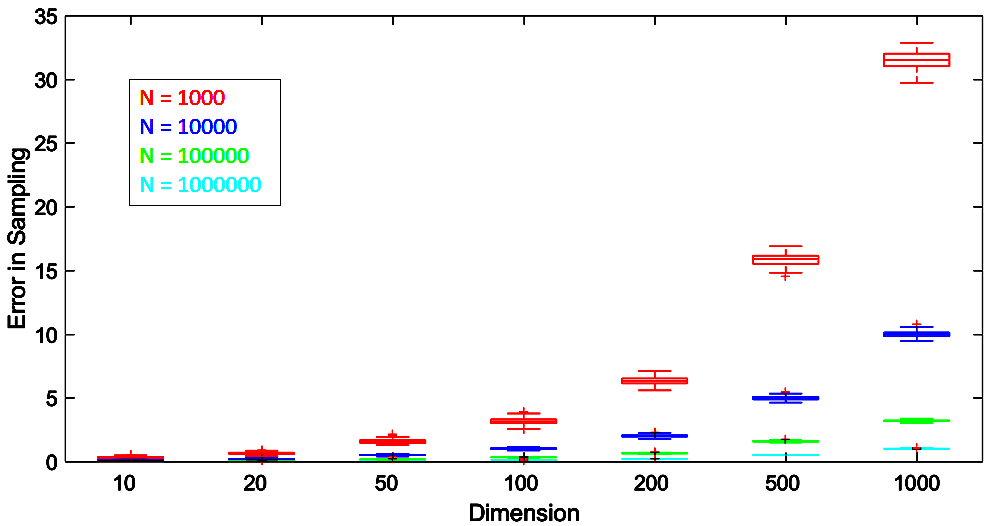
\includegraphics[width=\textwidth]{uq_figs/monte_linear}
\caption{}
\end{subfigure}
\caption{Error in Sampling by Monte Carlo sampling with dimension $n$ on (a) log scale and (b) linear scale}
\label{fig:monte_accuracy}
\end{figure}

%such as Monte Carlo Simulation~\cite{fishman1996monte}, Importance Sampling~\cite{melchers1989importance}, Quasi-Monte Carlo simulation~\cite{caflisch1998monte} 


% or quadrature based techniques such as Gaussian Quadrature~\cite{stroud1966gaussian}, Cubature~\cite{arasaratnam2009cubature}, Polynomial Chaos Expansion (PCE)~\cite{xiu2002wiener} may require huge amount of computation time, depending on the dimension of the problem. 

\begin{table}[H]
\begin{center}
\caption{List of some standard UQ methods}
\resizebox{\columnwidth}{!}{
\label{uq_methods}
\begin{tabular}{|l|l|l|}
\hline
Sampling-Based Methods& Examples \\ \hline
MC (pseudo-random number generator) &   Mersenne Twister~\cite{matsumoto1998mersenne}, LCG~\cite{marsaglia1972structure}, LFG~\cite{marsaglia1990toward} \\ \hline
Low-Discrepancy (Quasi-MC) &   Halton~\cite{halton1960efficiency}, Hammersley~\cite{hammersley2013monte}, Sobol~\cite{bratley1988algorithm}, van der Corput~\cite{der1935verteilungsfunktionen} \\ \hline
Stratified Sampling & LHS~\cite{iman2008latin} \\ \hline
Markov Chain MC Sampling & Metropolis-Hastings~\cite{hastings1970monte}, Gibbs~\cite{geman1984stochastic}, HMC~\cite{duane1987hybrid} \\ \hline
Other &  Importance Sampling~\cite{melchers1989importance} \\ \hline
\end{tabular} 
}
\end{center}
\end{table}

However, since all sampling methods are derived from the traditional Monte Carlo sampling, the linear accuracy trends for all of them are similar. 

\section{Quadrature-based Methods}

Quadrature (or Cubature for number of dimensions more than one) based methods involve a deterministic scheme to generate the set of $\mathcal{N}$ collocation points $\mathcal{X}_i$'s and associated weights $W_i$'s, such that the expectation integral in Equation~\ref{moment_whole} can be formulated as,

\begin{equation}
\label{quad_int}
E[\mathcal{G}(\textbf{x}_t)] = \int \int \ldots \int_{\Omega_{\textbf{x}}} \mathcal{G}(x_{t1},x_{t2},\ldots,x_{tn}) dP_{\textbf{x}} =  \sum_i^{\mathcal{N}} \mathcal{W}_i \mathcal{G}(\mathcal{X}_i)
\end{equation}

Setting all $W_i = 1/\mathcal{N}$ gives you Equation~\ref{monte_int}. However, unlike the MC methods, quadrature-based methods do not rely on any pseudo-random number generator. Instead, they use different classes of orthogonal polynomials to generate $(\mathcal{X},\mathcal{W})_i$'s via quadrature rule. The 1-D quadrature rule~\cite{stroud1966gaussian} states that, by suitably choosing suitable pair of $(\mathcal{X},\mathcal{W})_i$'s, the following 1-D integral equation can be solved exactly up to a polynomial degree of $2\mathcal{N} - 1$

\begin{equation}
E[g(x)] = \int_{\Omega_{x}} g(x) dP_x = \sum_i^{\mathcal{N}} g(\mathcal{X}_i) \mathcal{W}_i
\end{equation}

\noindent Setting $g(x) = \lbrace 1,x,x^2,\ldots,x^{2\mathcal{N} - 1} \rbrace$ the above equation becomes the 1-D moment constraint equation (MCE) as,

\begin{equation}
\label{mce_1d}
Q_d = E[x^d] = \int_{\Omega_x} \tau^d p_x(\tau) d \tau = \sum_i^{\mathcal{N}} \mathcal{X}_i^d \mathcal{W}_i \hspace{5mm} d = 0,1,\ldots,2\mathcal{N} - 1
\end{equation}

Instead, of solving the system of equations in~\ref{mce_1d}, the weight functions are assumed to belong to a suitable class of orthogonal polynomial of order $\mathcal{N}$. It can be shown that the collocation points $\mathcal{X}_i$'s are the roots of the particular $\mathcal{N}$-th order polynomial~\cite{press2007numerical}. The choice of this polynomial depends on the class of pdf involved in Equation~\ref{mce_1d} (For example use of Hermite polynomial for Gaussian pdf). Abramowitz and Stegun~\cite{abramowitz1964handbook} have listed a list of orthogonal polynomials (see Table~\ref{gauss_quad_pol}) and their roots. 

\begin{table}[H]
\begin{center}
\caption{1D Gauss Quadrature polynomials}
\label{gauss_quad_pol}
\resizebox{\textwidth}{!}{
\begin{tabular}{|c|c|c|c|}
\hline
$\Omega$ & Orthogonal Polynomial & Function & Quadrature Rule \\ \hline
$(-\infty,+\infty)$ & Hermite & $\exp(-x^2)$ & Gauss-Hermite \\ \hline
$[-1,1]$ & Legendre & $1$ & Gauss-Legendre \\ \hline
$[0,+\infty)$ & Laguerre & $x^a \exp(-x) $ & Gauss-Laguerre \\ \hline
$[-1,1]$ & Chebyshev & $1/\sqrt{1-x^2}$ & Gauss-Chebyshev \\ \hline
$[-1,1]$ & Jacobi & $(1-x^a)(1+x^b), a,b > -1 $ & Gauss-Jacobi \\ \hline
\end{tabular}
}
\end{center}
\end{table}

Cubature method (quadrature for $n>1$) is an extension of the 1-D Gaussian quadrature method, whereby instead of solving the 1D MCE in Equation~\ref{mce_1d}, the pair of collocation points and weights $(\mathcal{X},W)_i$'s can exactly produce moments of a multivariate polynomial functions up to order $d$, by solving the following n-dimensional MCE:

\begin{equation}
\label{mce_nd}
Q_d^n = \sum_{i=1}^{\mathcal{N}_d} w_i \lbrace x_1^{m_1} \ldots x_n^{m_n} \rbrace = E \left[ x_1^{m_1},\ldots,x_n^{m_n}  \right]  \hspace{5mm} m_1 + m_2 + \ldots m_n \leq d
\end{equation}

\subsection{Gaussian Cubature}

Gaussian cubature~\cite{arasaratnam2009cubature}, also termed as product rule is generated by taking the tensor product of the 1D quadrature rule explained above. Given a multivariate pdf $p(\textbf{x}) = \lbrace x_1, \ldots, x_n \rbrace$, $\textbf{x} \in \mathbb{R}^n$, the first step is to generate $\mathcal{N}$ collocation points and weights $(\mathcal{X}_j,\mathcal{W}_j)_i$ for each variable $x_J$ to approximate polynomial integral up to degree $2\mathcal{N} - 1$. Next, the set of collocation points for $\textbf{x}$ is generated by taking the tensor product of all $\mathcal{X}_j$ set of points by the following integral equation

\begin{equation}
\label{eqn:gauss_quad}
Q_d^n = Q_d^1 \otimes Q_d^2 \otimes \ldots \otimes Q_d^n
\end{equation}

Thus the number of points generated is $\mathcal{N}_n = \mathcal{N}^n$. The associated weights are formulated as,

\begin{equation}
W_i = W_{1i}W_{2i} \ldots W_{ni} \ldots i = 1,2,\ldots,\mathcal{N}_n
\end{equation}

It is evident that this method suffers from the curse of dimensionality as the required number of points grows exponentially with the dimension $n$ (see Figure~\ref{fig:gauss_quad} for a given value of $d$ as per Equation~\ref{mce_nd}. 

\begin{figure}[H]
\centering
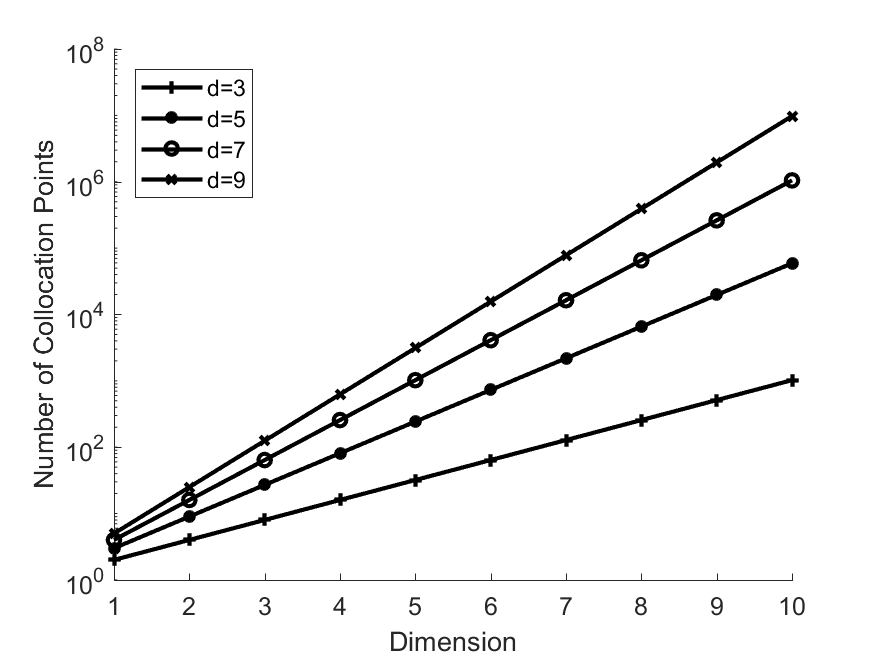
\includegraphics[width=\textwidth]{intr_figs/gauss_hermite}
\caption{Number of Collocation Points vs Dimension $n$ for different values of $d$ in Equation~\ref{mce_nd} using Gauss-Hermite class of Orthogonal Polynomial}
\label{fig:gauss_quad}
\end{figure}


\subsection{Sparse-Grid Collocation}

Sparse-Grid or Smolyak collocation techniques generates the cubature rule by invoking a sparse tensor product unlike the Gaussian cubature to reduce the number of monomials involved in the integral calculation of Equation~\ref{monte_int}. The number of monomials involved in Equation~\ref{eqn:gauss_quad} is $\binom{n+d}{n}$ that grows exponentially with $n$ for a given $d$. Smolyak observed that the key to reducing the number of collocation points lie in the number of monomials involved for the integral computation. The first step of generating collocation points is similar to 1D quadrature method of solving Equation~\ref{mce_1d}. The integral equation in~\ref{mce_nd} for a given $d$ can be written in a recursive formulation as~\cite{gerstner1998numerical},

\begin{equation}
\label{mce_sparse}
Q_k^n = \sum_i^k (Q_i^1 - Q_{i-1}^1) \otimes Q^{n-1}_{k-i+1} 
\end{equation}

\noindent where, $d=2k-1$, $Q_n^1$ is the univariate quadrature rule and $Q_0^1 = \emptyset$. Under this transformation in Equation~\ref{mce_sparse}, the number of collocation points comes out to be less than that required by the product in Equation~\ref{eqn:gauss_quad}. However, the required number of collocation points still grows exponentially with the size of the problem (see Figure~\ref{fig:gauss_quad_sparse}). 

\begin{figure}[H]
\centering
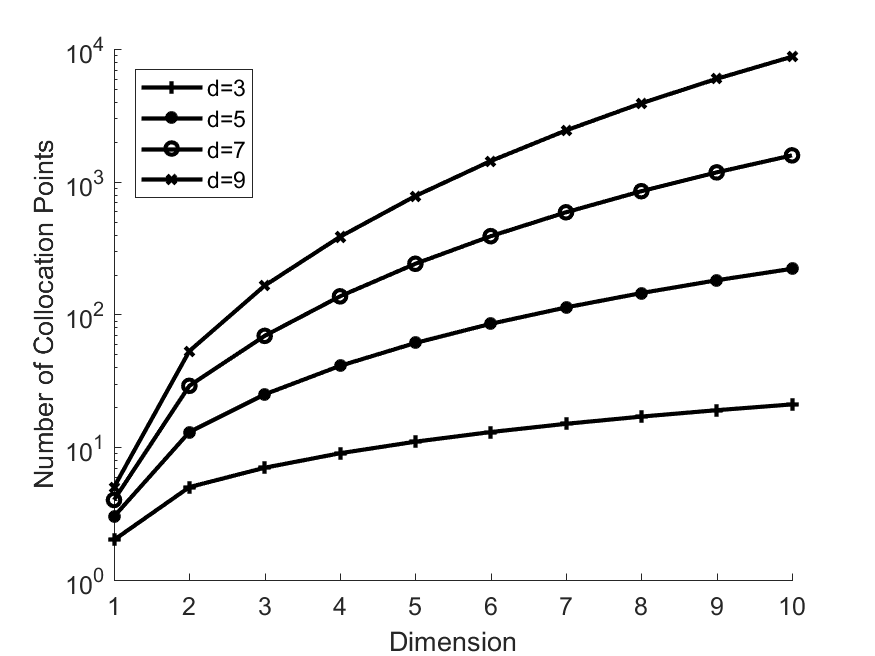
\includegraphics[width=\textwidth]{intr_figs/gauss_hermite_sparse}
\caption{Number of Collocation Points vs Dimension $n$ for different values of $d$ in Equation~\ref{mce_sparse} using Gauss-Hermite class of Orthogonal Polynomial}
\label{fig:gauss_quad_sparse}
\end{figure}

\subsection{Minimal Cubature Rules}

For faster computation of the integral Equation~\ref{mce_nd} maintaining the same exactness, cubature rules have been proposed that optimally chooses the number of collocation points $N$ depending on $n$, $d$, choice of the pdf $p(x)$ and also the domain of integral $\Omega_{\textbf{x}}$. A list of minimal cubature rules can be listed in Refs~\cite{stroud1971approximate,cools2003encyclopaedia,Cools1}. Readers are also advised to check Ref~\cite{cubatureurl} for tabulated form of different cubature rules along with their references. An excerpt of the table for Gaussian weight function is given in Table~\ref{tab:cubature}.

\begin{table}
\begin{center}
\caption{Cubature formula with weight function $\exp(-\textbf{x}^T\textbf{x})$, $\textbf{x} \in \mathbb{R}^n$}
\label{tab:cubature}
\begin{tabular}{|c|c|c|}
\hline
$d$ & $N$ & $n$ \\ \hline
3  & $2n$ & all dimensions \\ \hline
3  & $2^n$ & all dimensions \\ \hline
5  & $n^2 + n + 2$ & $2 \leq n \leq 7$ \\ \hline
5  & $2^{n+1} - 1$ & all dimensions \\ \hline
7  & $2^n + 2n^2 + 1$ & $3 \leq n \leq 7$ \\ \hline
7  & $ ( 4n^3 + 12n^2 - 4n + 3 ) / 3$ & all dimensions \\ \hline
9  & $( 2n^4 - 4n^3 + 22n^2 - 8n + 3 ) / 3$ & $n \geq 4$ \\ \hline
11  & $( 4n^5 - 20n^4 + 140n^3 - 130n^2 + 96n + 15 ) / 15$ & all dimensions \\ \hline
\end{tabular}
\end{center}
\end{table}

\subsection{Unscented Transform}

Unscented Transform~\cite{julier1997new} is fast and accurate UQ method for problems with Gaussian variables. Given, at a time instance, the state variable $\mathbf{x}_{t_k}$ is Gaussian, UT generates sample points $\mathcal{X}_i$ and associated weights $W_i$ that can accurately estimate the moments of the Gaussian variable up to the order 2. In other words, the sample points $\mathcal{X}_i$ satisfy the moment constraint equations given in Equation~\ref{mce_nd}. Here, $m_1 + m_2 + \ldots m_n = 2$. Given the distribution of $\textbf{x}_t \sim \mathcal{N}(\bm{\mu}_{t_k},\Sigma_{t_k})$, UT uses a deterministic technique to generate the sigma points $\mathcal{X}$ and the related weights $W$ as~\cite{julier1997new}:
\begin{equation}
\label{sigmapt}
\begin{array}{lr}
\mathcal{X}_0 = \bm{\mu}_{t_k} &W_0 = \kappa /(n+ \kappa)  \\
\mathcal{X}_i = \bm{\mu}_{t_k} + \left( \sqrt{(n+ \kappa) \Sigma_{t_k}} \right)_i  &W_i = 1 /2(n+ \kappa)  \\
\mathcal{X}_{i+n} = \bm{\mu}_{t_k} - \left( \sqrt{(n+ \kappa) \Sigma_{t_k}} \right)_i  &W_{i+n} = 1 /2(n+ \kappa)
\end{array}
\end{equation}
$\left( \sqrt{(n+ \kappa) \Sigma_{t_k}} \right)_i$ is the $i$th row or column of the matrix square root of $(n+ \kappa) \Sigma_{t_k}$. For the numerical examples, the value of $(n+\kappa)$  has been taken to be 3. These sigma points are then propagated by the flow map $\phi^t(\mathcal{X})$ as defined in Eqn.~\ref{stochflow}. The mean and the variance of the propagated points at time $t_{k+1}$ is given by,
\begin{equation}
\label{prop}
\begin{array}{l}
\bm{\mu}_{t_{k+1}} =  \displaystyle \sum_{i=1}^{2n+1} W_i \mathcal{X}_i   \\
\Sigma_{t_{k+1}} = \displaystyle \sum_{i=1}^{2n+1} W_i (\mathcal{X}_i - \bm{\mu}_{t_{k+1}})(\mathcal{X}_i - \bm{\mu}_{t_{k+1}})^T  \notag
\end{array}
\end{equation}
\begin{figure}[H]
\centering
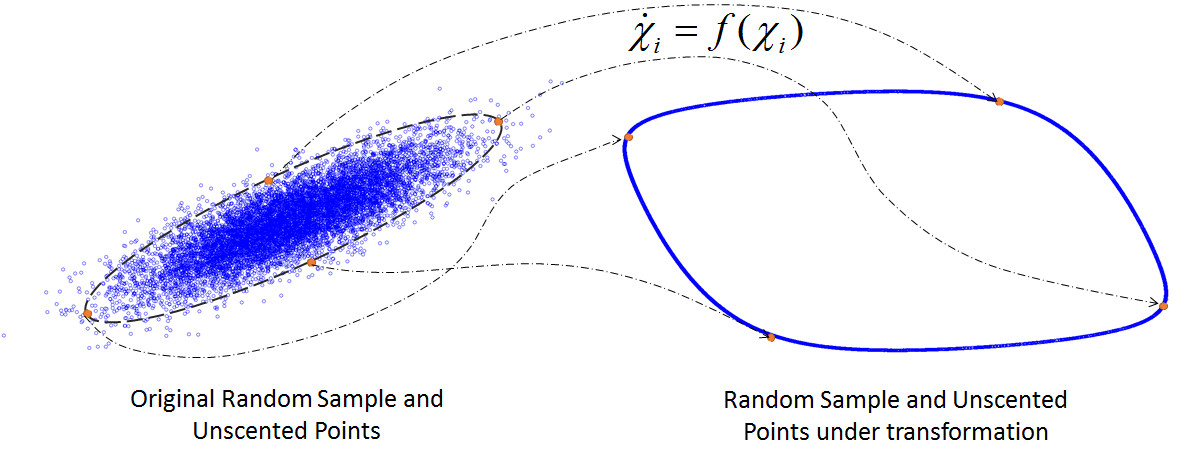
\includegraphics[width=\textwidth]{figures/FIG_9}
\caption{Working of the Unscented Transformation}
\label{UnscT}
\end{figure}

Figure~\ref{UnscT} shows the analogy between Monte-Carlo samples and UT sigma points, which are generated from the initial distribution space and then are propagated through the dynamical flow equation.

\subsection{Other Methods}

Prior work related to Uncertainty Quantification (UQ) in nonlinear systems is mostly limited to efficiently solving small-scale problems~\cite{mezic2008uncertainty,demars2013entropy,fujimoto2012analytical}. For large scale systems, UQ methods based on decoupling entire state space into interconnected smaller state spaces 
have been recently pursued~\cite{callier1976input,georgiou1992linear,varigonda2004graph,dellnitz2003congestion,surana2012iterative}. A fundamental limitation of these existing works is the approximation of the nonlinear nature of the system through the use of Jacobian at the initial condition.

A summary of all the methods show that, it is hard to obtain a method that works for any degree $d$ and for any dimension $n$. Product-rule based Gaussian cubature and Smolyak-grid collocation method shows exponential requirement of collocation points. The cubature rules in Table~\ref{tab:cubature} exist for certain dimension $n$ and for any degree of polynomial approximation $d$. Linear requirement of collocation points $N$ exist only for $d=3$. For other $d$'s, $N$ varies either in polynomial or exponential order. Such a requirement can scale up fast for high-dimensional problems.
Despite the effectiveness, the approaches mentioned above still requires significant computation time while tackling scalable high-dimensional problems. For such methods, it is imperative to incorporate a clustering method with any of the UQ techniques, to achieve the same efficiency for a lesser computational time. 